%% Methods + Results + floats for the CRSD paper (\input by main.tex).

\section{Methods}

\subsection{The collective-risk climate dilemma}
We replicate the collective-risk social dilemma (CRSD) of \textcite{milinski2008climate}. Six players each receive a private endowment of €40 and play ten rounds. In every round each player simultaneously and privately invests €0, €2 or €4 into a shared climate account; the climate cover story matches the original. The group must accumulate a cumulative target of €120 across all players and rounds. If the target is reached, each player keeps €40 minus their own total investment; if it is missed, a single group-level lottery is drawn in which, with loss probability $p$, every player loses everything (final payoff €0), and otherwise each keeps their remainder. The catastrophe risk $p$ is crossed at three levels, $p\in\{90\%,50\%,10\%\}$, which constitutes the diagnostic manipulation of the design. There is no communication. Faithful to the original ``took notes by hand'' visibility, players observe one another's per-round contributions under fixed anonymous identifiers but are never shown the running cumulative total; the maximum attainable group total is €240 (six players each investing €4 in all ten rounds), twice the target. We run ten independent groups per cell.

\subsection{Agents, models and protocol}
Each agent is an instruction-tuned LLM that receives a single natural-language prompt comprising a brief of the game rules, the history of play so far, and a disposition block, after which it reasons briefly and emits a parseable decision line of the form \texttt{CONTRIBUTION = X} (with $X$ one of 0, 2 or 4). Within each round, all six agents' decisions are collected in a single lockstep batch so that play is genuinely simultaneous. The protocol is built on the FAIRGAME multi-agent framework \parencite{fairgame2025}. We serve three open-weight instruction-tuned models, Qwen2.5-7B-Instruct \parencite{qwen2025}, Gemma-2-9B-it \parencite{gemma2024} and Llama-3.1-8B-Instruct \parencite{llama2024}, via vLLM at temperature 0.8 with a fixed seed to make runs reproducible; all simulations were executed offline on a single RTX PRO 6000. Exact model identifiers, decoding settings and per-condition game counts are listed in the electronic supplementary material. We cross the game with five languages (English, French, Arabic, Chinese, Vietnamese) and four dispositional prompts (neutral, cooperative, selfish, risk-averse), each rendered as a short instruction prepended to the brief (the neutral prompt adds no disposition).

\subsection{Measures and analysis}
For each game we record whether the €120 target was reached (success), the final group total, and the number of ``fair-sharers'' per group, defined as players whose total contribution is at least €2 per round on average (i.e.\ at least €20 over the ten rounds), matching Milinski's notion of a fair share. The central diagnostic is the model's sensitivity to the loss-probability manipulation, which we test with a one-way ANOVA of the final group total across the three treatments, computed separately per model and benchmarked against the human ANOVA ($F=13.78$, $P<0.0001$); model success rates are compared with the human baseline using Fisher's exact test and group totals using Welch's $t$-test. Each significance test is accompanied by a bias-corrected effect size (Hedges $g$ for the mean contrasts) with 95\%\ confidence intervals, and the family-wise error rate across the nine baseline cells is controlled with the Holm--Bonferroni procedure; the full effect-size tables appear in the electronic supplementary material. Throughout, we log the \texttt{parse\_fallback} (format non-compliance) rate for every cell and report it as a joint data-quality and fairness signal, since it varies systematically across languages. Finally, because agents are shown each player's per-round contributions but never the running cumulative total, any apparent target tracking must arise from the model's own arithmetic self-summation across the visible history rather than from a displayed total; we treat this requirement as a caveat when interpreting the models' near-uniform attainment of the target.

\section{Results}

\begin{table*}[t]
\caption{Behaviour of the three LLM agents in the faithful baseline (English
prompt, neutral disposition) against the human benchmark of Milinski
\textit{et al.}\ \cite{milinski2008climate}, by loss probability. ``Target
reached'' is the fraction of the ten groups whose cumulative investment met the
€120 threshold; ``Final total'' is the mean group investment ($\pm$ s.e.m.);
``Fair-sharers'' is the mean number of group members (of six) investing at least
€2 per round on average. All LLM-versus-human contrasts are significant (Welch
$t$ on totals and Fisher exact on success, all $p<0.05$).}
\label{tab:baseline}
\centering
\begin{tabular}{llccc}
\toprule
Loss prob. & Player & Target reached & Final total (€) & Fair-sharers \\
\midrule
\multirow{4}{*}{90\%}
 & Human \cite{milinski2008climate} & 50\%  & 118.2 & 3.3 \\
 & Qwen2.5-7B   & 100\% & 183.0 $\pm$ 2.1 & 6.0 \\
 & Gemma-2-9B   & 100\% & 168.2 $\pm$ 3.3 & 5.8 \\
 & Llama-3.1-8B & 100\% & 177.4 $\pm$ 2.9 & 5.8 \\
\midrule
\multirow{4}{*}{50\%}
 & Human \cite{milinski2008climate} & 10\%  & 92.2  & 2.1 \\
 & Qwen2.5-7B   & 100\% & 186.6 $\pm$ 1.2 & 6.0 \\
 & Gemma-2-9B   & 100\% & 162.8 $\pm$ 2.9 & 5.9 \\
 & Llama-3.1-8B & 100\% & 165.2 $\pm$ 3.6 & 5.6 \\
\midrule
\multirow{4}{*}{10\%}
 & Human \cite{milinski2008climate} & 0\%   & 73.0  & 1.1 \\
 & Qwen2.5-7B   & 100\% & 181.0 $\pm$ 2.8 & 5.9 \\
 & Gemma-2-9B   & 100\% & 158.0 $\pm$ 3.9 & 5.8 \\
 & Llama-3.1-8B & 100\% & 170.0 $\pm$ 3.1 & 5.7 \\
\bottomrule
\end{tabular}
\end{table*}

\begin{figure*}[t]
\centering
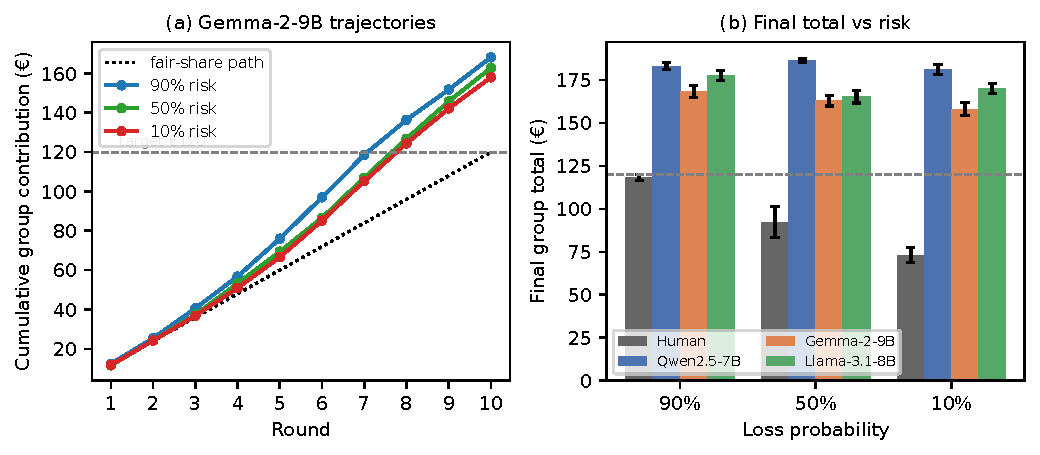
\includegraphics[width=\textwidth]{figures/fig1_risk.pdf}
\caption{Over-cooperation and insensitivity to catastrophe risk.
(\textit{a}) Cumulative group investment per round for Gemma-2-9B at the three
loss probabilities, against the fair-share path and the €120 target; the three
risk curves nearly coincide and all cross the target. (\textit{b}) Final group
total by loss probability for humans \cite{milinski2008climate} and the three
LLMs: humans fall steeply as catastrophe risk declines (one-way ANOVA
$F=13.78$, $p<0.0001$), whereas every model stays flat and far above target
(model ANOVA $F=1.76$/$2.23$/$3.64$). Error bars are s.e.m.}
\label{fig:risk}
\end{figure*}

In the human collective-risk dilemma, the loss probability is the lever that separates prudent from reckless groups: only half of Milinski's groups reached the €120 climate target under the gravest 90\% catastrophe risk, one in ten reached it at 50\%, and none reached it at 10\%, with final group totals falling from €118 through €92 to €73 as the threat receded \cite{milinski2008climate}. The LLM agents show no such restraint. In the English, neutral baseline, all three models---Qwen2.5-7B-Instruct, Gemma-2-9B-it and Llama-3.1-8B-Instruct---reach the target on 100\% of games at every loss probability (table~\ref{tab:baseline}), and they do so by over-investing rather than by tracking the threat: final group totals cluster between roughly €158 and €187, some 70--78\% of the €240 ceiling attainable if every player invested the maximum in every round, and far above the human totals of €118, €92 and €73. The same over-supply is visible in the count of ``fair-sharers'': where human groups typically contained only one to three players investing at least €20 over the game, the model groups contain roughly six of six. Welch tests on final totals and Fisher exact tests on success counts confirm that these model--human gaps are statistically significant across the board (table~\ref{tab:baseline}).

The decisive diagnostic, however, is not the level of cooperation but its insensitivity to risk. In humans the loss-probability manipulation is what drives behaviour, producing a steep and monotone decline (one-way ANOVA across the three treatments $F=13.78$, $P<0.0001$). The models reproduce none of this gradient: the analogous ANOVA on final group totals yields only $F=1.76$ ($P=0.19$) for Qwen, $F=2.23$ ($P=0.13$) for Gemma and $F=3.64$ ($P=0.040$) for Llama, and even the lone nominally significant case is weak and non-monotone rather than the orderly human descent. Figure~\ref{fig:risk}a makes the failure concrete: the cumulative-contribution trajectories for 90\%, 50\% and 10\% loss risk nearly coincide and all cross the €120 target well before the final round, regardless of how much is actually at stake. Figure~\ref{fig:risk}b sharpens the contrast by plotting final total against loss probability: the human line falls steeply as catastrophe risk recedes, whereas all three model lines stay essentially flat and far above target. The manipulation that makes the experiment informative about human risk preferences leaves the models almost untouched.

\begin{figure*}[t]
\centering
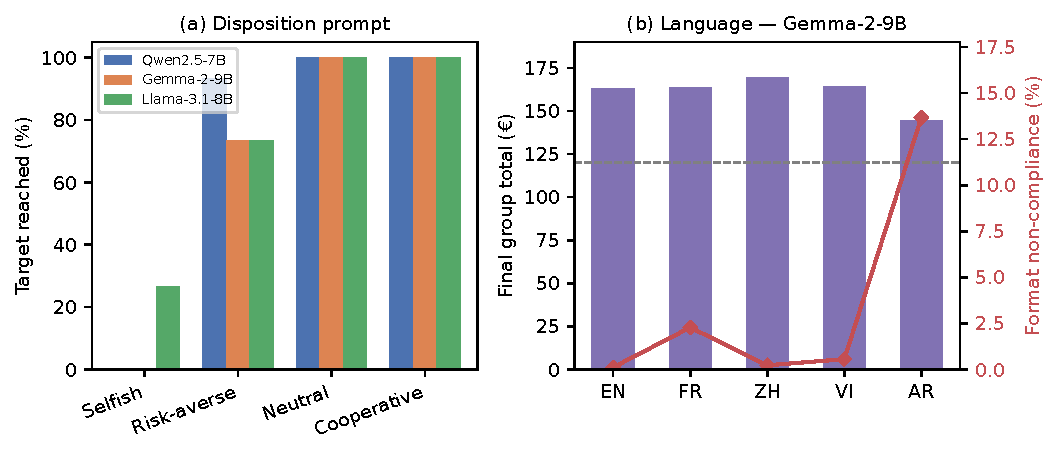
\includegraphics[width=\textwidth]{figures/fig2_moderators.pdf}
\caption{Moderators of the over-cooperation result. (\textit{a}) Target-success
rate by dispositional prompt: a ``selfish'' instruction collapses cooperation
(0\% success for Qwen and Gemma), ``risk-averse'' is intermediate, and
``neutral''/``cooperative'' sit at the ceiling, showing that the default
high-prosociality behaviour is a steerable knob. (\textit{b}) Gemma-2-9B final
total (bars) and format non-compliance rate (line) by prompt language:
cooperation is broadly language-invariant in content, but format reliability
degrades sharply in Arabic.}
\label{fig:moderators}
\end{figure*}

That the default behaviour is a high-prosociality persona rather than a fixed trait becomes clear once disposition is varied. The dispositional prompt is a powerful lever on the same models (figure~\ref{fig:moderators}a): switching the agents from neutral to a selfish disposition collapses target success from the ceiling to 0\% for Qwen and Gemma and to 27\% for Llama, with final group totals dropping into the €33--113 range and many groups now missing the target outright. A risk-averse disposition produces an intermediate regime (success between 73\% and 93\%), while the neutral and cooperative prompts both sit at or near the 100\% ceiling. The behaviour therefore moves across almost the entire feasible range under prompt control, which indicates that the over-cooperative baseline reflects a steerable default persona rather than an immovable property of the architecture---a knob, not a trait.

Finally, the core result is robust across languages while exposing a low-resource fragility that is a fairness caveat rather than an explanation. Translating the game into French, Chinese, Vietnamese and Arabic leaves the substantive outcomes roughly invariant: the models still over-cooperate and still ignore the risk gradient. What does vary is format compliance. The rate of format non-compliance (parse-fallback) stays below 2.5\% in most cells but spikes to 13.7\% for Gemma in Arabic and 14.8\% for Llama in Vietnamese (figure~\ref{fig:moderators}b), a non-trivial degradation that the framework logs as a data-quality and fairness signal. Crucially, the English baseline that carries the over-cooperation result has a parse-fallback rate of essentially 0\%, so the failure to track risk cannot be dismissed as an arithmetic or parsing artefact: the models read the game correctly and still pour in resources regardless of the odds.
